%!TEX TS-program = xelatex
%!TEX encoding = UTF-8 Unicode

\documentclass[12pt]{extarticle}
% extarticle is like article but can handle 8pt, 9pt, 10pt, 11pt, 12pt, 14pt, 17pt, and 20pt text

\def \ititle {Origins of Mind}

\def \isubtitle {Lecture 01}

\def \iauthor {Stephen A. Butterfill}
\def \iemail{s.butterfill@warwick.ac.uk}
\date{}

%for strikethrough
\usepackage[normalem]{ulem}

\input{$HOME/Documents/submissions/preamble_steve_handout}

%\bibpunct{}{}{,}{s}{}{,}  %use superscript TICS style bib
%remove hanging indent for TICS style bib
%TODO doesnt work
\setlength{\bibhang}{0em}
%\setlength{\bibsep}{0.5em}


%itemize bullet should be dash
\renewcommand{\labelitemi}{$-$}

\begin{document}

\begin{multicols*}{3}

\setlength\footnotesep{1em}


\bibliographystyle{newapa} %apalike

%\maketitle
%\tableofcontents




%---------------
%--- start paste





\def \ititle {Lecture 07: Mindreading in Humans}

\begin{center}

{\Large

\textbf{\ititle}

}



\iemail %

\end{center}



\section{Automatic Belief-tracking}

Are human adults’ abilities to track others’ beliefs automatic?

For our purposes, a process is \emph{automatic} to the degree that whether it occurs is independent of
its relevance to the particulars of the subject's task, motives and aims.

‘Automatic mindreading’ is short for ‘mindreading that is a consequence of
automatic processes only.’

\citet{Southgate:2007js} created an anticipatory looking false belief task, originally
for use with two-year-olds, which has been adapated to provide evidence for automatic
false belief tracking.

There is evidence that some mindreading in human adults is
entirely a consequence of relatively automatic processes
\citep{kovacs_social_2010,Schneider:2011fk,Wel:2013uq} and
that not all mindreading in human adults is
\citep{apperly:2008_back,apperly:2010_limits,Wel:2013uq}.

‘Participants never reported belief tracking when questioned in an open format after the experiment
(“What do you think this experiment was about?”). Furthermore, this verbal debriefing about the
experiment’s purpose never triggered participants to indicate that they followed the actor’s belief
state’ \citep[p.~2]{Schneider:2011fk}

\emph{Dual Process Theory of Mindreading}.
Automatic and nonautomatic mindreading processes are independent in
this sense: different conditions influence whether they occur and
which ascriptions they generate.

\citet{qureshi:2010_executive} found that automatic and nonautomatic
mindreading processes are differently influenced by cognitive load, and
\citet{todd:2016_dissociating} provided evidence that adding time pressure
affects nonautomatic but not automatic mindreading processes.

\citet{lin:2010_reflexively} show that successful visual perspective taking (in the
director task) is faster among those with greater working memory capacity (Experiment 1) and
slower when cognitive load is imposed (Experiment 2).



\section{Minimal Theory of Mind}

An agent’s \emph{field} is a set of objects related to the agent by proximity, orientation and other factors.

First approximation: an agent \emph{encounters} an object just if it is in her field.

A \emph{goal} is an outcome to which one or more actions are, or might be, directed.

%(Not to be confused with a \emph{goal-state}, which is an intention or other state of an agent linking an action to a particular goal to which it is directed.)

\textbf{Principle 1}: one can’t goal-directedly act on an object unless one has encountered it.

Applications: subordinate chimps retrieve food when a dominant is not informed of its
          location \citep{Hare:2001ph}; when observed scrub-jays prefer to cache in shady, distant and
          occluded locations \citep{Dally:2004xf,Clayton:2007fh}.

First approximation: an agent \emph{registers} an object at a location just if she most recently encountered the object at that location.

A registration is \emph{correct} just if the object is at the location it is registered at.

\textbf{Principle 2}: correct registration is a condition of successful action.

Applications: 12-month-olds point to inform depending on their informants’ goals and ignorance \citep{Liszkowski:2008al};
          chimps retrieve food when a dominant is misinformed about its location \citep{Hare:2001ph};
          scrub-jays observed caching food by a competitor later re-cache in private \citep{Clayton:2007fh,Emery:2007ze}.

\textbf{Principle 3}: when an agent performs a goal-directed action and the goal specifies an object, the agent will act as if the object were actually in the location she registers it at.

Applications: some false belief tasks \citep{Onishi:2005hm,Southgate:2007js,Buttelmann:2009gy}.



\section{Signature Limits}

Automatic belief-tracking in adults and
belief-tracking in infants are both subject to signature limits
associated with minimal theory of mind
(\citealp{wang:2015_limits,Low:2012_identity,low:2014_quack,mozuraitis:2015_privileged};
contrast \citealp{scott:2015_infants}).

\begin{center}

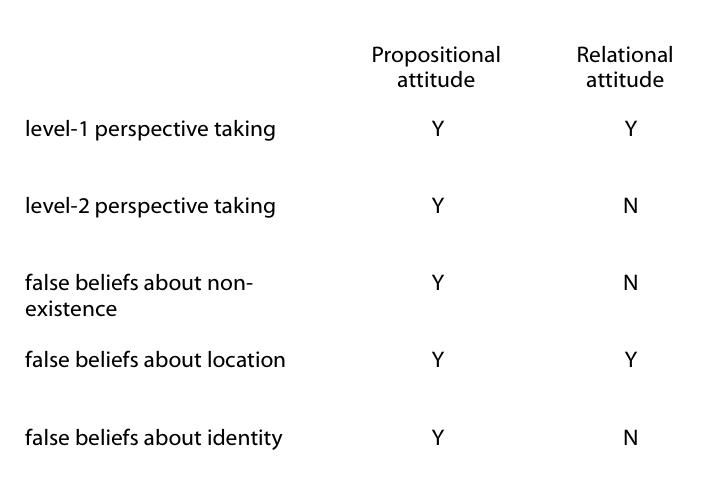
\includegraphics[width=0.25\textwidth]{fig/signature_limits_table.png}

\end{center}

\begin{center}

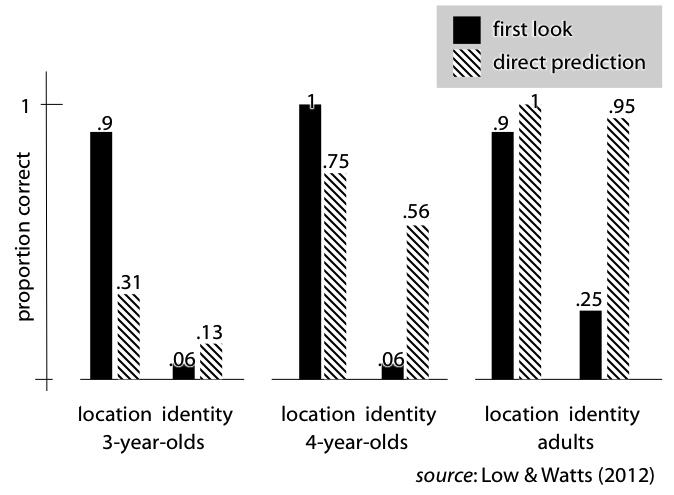
\includegraphics[width=0.3\textwidth]{fig/low_2012_fig.png}

\end{center}

For adults (and children who can do this),
representing perceptions and beliefs as such---and even merely holding in mind
what another believes, where no inference is required---involves a measurable
processing cost \citep{apperly:2008_back,apperly:2010_limits}, consumes attention
and working memory in fully competent adults \citealp{Apperly:2009cc,
lin:2010_reflexively, McKinnon:2007rr},  may require inhibition \citep{bull:2008_role}
and makes demands on executive function \citep{apperly:2004_frontal,samson:2005_seeing}.

Objection:
‘the theoretical arguments offered [...] are [...] unconvincing, and [...]
the data can be explained in other terms’
(\citealp{carruthers:2015_two}; see also \citealp{carruthers:2015_mindreading}).

‘A cooperative multi-system architecture is better able to explain infant belief representation than a
parallel architecture, and causal representation, schemas and models provide a more promising basis
for flexible belief representation than does a rule-based approach of the kind described by Butterfill
and Apperly’ (\citealp{christensen:_twoa}; see also \citealp{michael:2016_flexible,michael:2013_mindreading}).


    



%--- end paste
%---------------

\footnotesize
\bibliography{$HOME/endnote/phd_biblio}

\end{multicols*}

\end{document}
